\documentclass{article}

\usepackage{graphicx}
\usepackage{tikz}
\usepackage{tikzsymbols}
\usetikzlibrary{calc,patterns,shapes.geometric}
\pagestyle{empty}
\usepackage[margin=0pt]{geometry}
\geometry{papersize={14in,12in}}

\def\centerarc[#1](#2)(#3:#4:#5){\draw[#1] ($(#2)+({#5*cos(#3)},{#5*sin(#3)})$) arc (#3:#4:#5);}

\begin{document}
	\begin{figure}
		\centering
		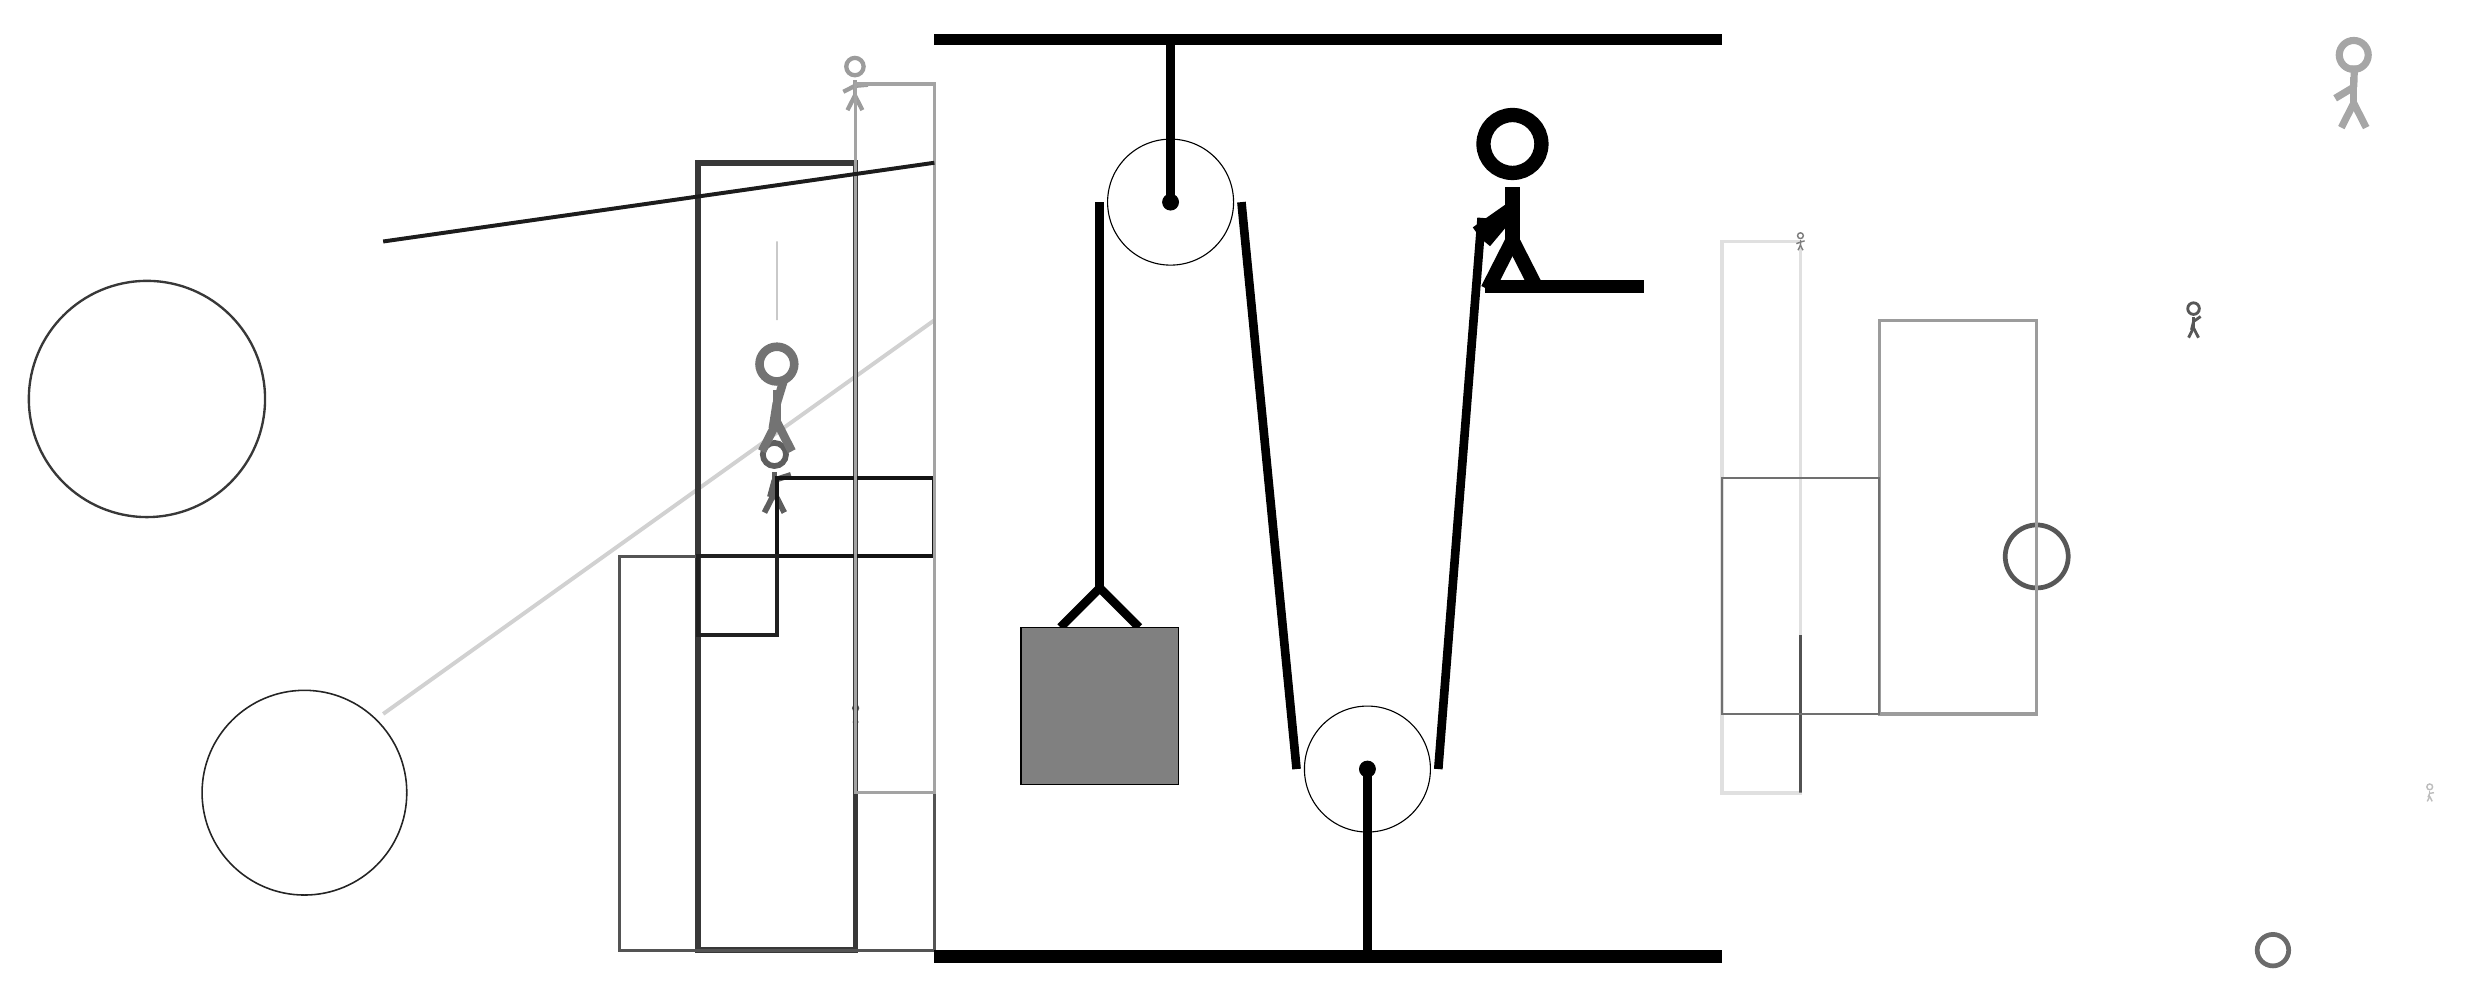
\begin{tikzpicture}
			%%%%% START %%%%%
			
			\draw[fill=black] (-2, 11.5) rectangle (8, 11.625);
			
			\draw (3.5, 2.3) circle (0.8);
			\draw[fill=black] (3.5, 2.3) circle (0.1);
			\draw[line width=1.1mm] (3.5, 2.3) -- (3.5, 0);
			
			\draw (1, 9.5) circle (0.8);
			\draw[fill=black] (1, 9.5) circle (0.1);
			\draw[line width=1.1mm] (1, 11.5) -- (1, 9.5);
			
			\draw[line width=1.1mm](-0.4, 4.1) --  (0.1, 4.6) -- (0.6, 4.1);
			\draw[fill=black!50] (-0.9, 4.1) rectangle (1.1, 2.1);
			
			\draw[line width=1.1mm](0.1, 9.5) -- (0.1, 4.6);
			\centerarc[line width=1.1mm](1, 9.5)(180:0:0.9)
			\draw[line width=1.1mm](1.9, 9.5) -- (2.6, 2.3);
			\centerarc[line width=1.1mm](3.5, 2.3)(180:360:0.9)
			\draw[line width=1.1mm](4.4, 2.3) -- (4.95, 9.3);
			
			\node at (5.3, 9.5) {\Strichmaxerl[10][35][-130]};
			\draw[fill=black] (5, 8.5) rectangle (7, 8.35);
			
			\node[line width=0.2mm, color=black!69] at (-3, 3) {\Strichmaxerl[1][89][69]};
			
			\draw[line width=0.5mm, color=black!18](-2, 8) -- (-9, 3);
			\draw [line width=0.6mm, color=black!66](12, 5) circle (0.4);
			\draw[line width=0.5mm, color=black!12] (9, 9) rectangle (8, 2);
			
			\draw[line width=0.5mm, color=black!16](-5, 4) -- (-4, 4);
			
			\node[line width=0.7mm, color=black!39] at (-3, 11) {\Strichmaxerl[3][27][5]};
			\node[line width=0.2mm, color=black!66] at (14, 8) {\Strichmaxerl[2][76][35]};
			\draw[line width=0.7mm, color=black!78] (-3, 0) rectangle (-5, 10);
			\node[line width=0.5mm, color=black!26] at (17, 2) {\Strichmaxerl[1][67][8]};
			
			\draw [line width=0.6mm, color=black!58](15, 0) circle (0.2);
			\draw[line width=0.3mm, color=black!21] (-4, 8) rectangle (-4, 9);
			
			\node[line width=0.6mm, color=black!63] at (-4, 6) {\Strichmaxerl[4][75][18]};
			\draw[line width=0.4mm, color=black!39] (10, 8) rectangle (12, 3);
			
			\draw[line width=0.4mm, color=black!67] (-2, 5) rectangle (-6, 0);
			\draw[line width=0.5mm, color=black!92] (-4, 5) rectangle (-2, 6);
			\draw[line width=0.5mm, color=black!68] (9, 4) rectangle (9, 2);
			
			\node[line width=0.2mm, color=black!51] at (9, 9) {\Strichmaxerl[1][21][17]};
			
			\draw[line width=0.4mm, color=black!36] (-2, 2) rectangle (-3, 11);
			\draw[line width=0.5mm, color=black!89](-2, 10) -- (-9, 9);
			\node[line width=0.3mm, color=black!55] at (-4, 7) {\Strichmaxerl[6][81][73]};
			\draw[line width=0.5mm, color=black!87] (-4, 4) rectangle (-5, 5);
			\draw [line width=0.3mm, color=black!78](-12, 7) circle (1.5);
			\draw[line width=0.3mm, color=black!56] (8, 3) rectangle (10, 6);
			\draw [line width=0.2mm, color=black!86](-10, 2) circle (1.3);
			\node[line width=0.5mm, color=black!35] at (16, 11) {\Strichmaxerl[5][31][88]};
			
			\draw[fill=black] (-2, 0) rectangle (8, -0.15);
			
			%%%%% END %%%%%
		\end{tikzpicture}
	\end{figure}	
\end{document}